\anexo
%% TEXTOS ABAIXO SÂO ANEXOS.
        
\chapter{Algo interessante que alguém fez}
         \par Algo como anexo.
         
          \begin{verbatim}
	    \begin{ilustracao}[ht]
		\centering
		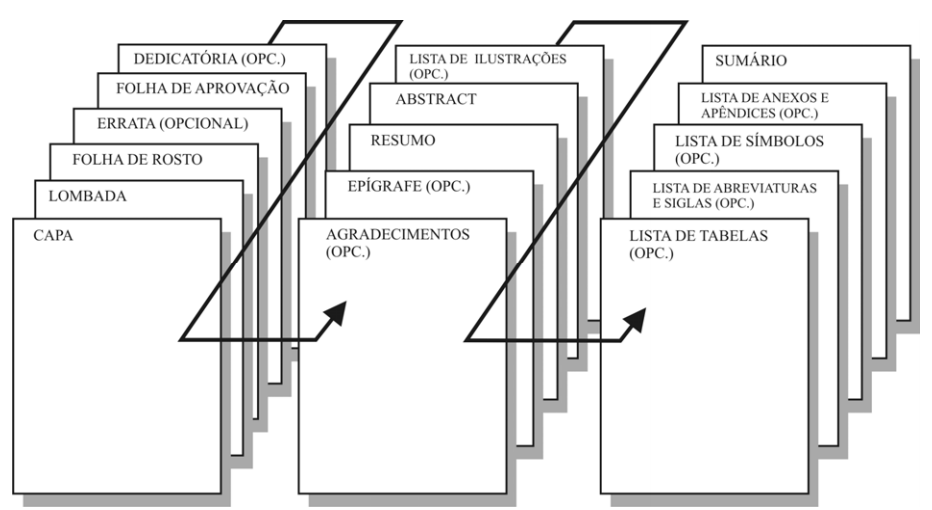
\includegraphics[width=0.6\textwidth]{figuras/pretextuais.png}
		\caption{\label{exepretex} Sequência dos elementros pré-testuais da MDT-UFSM}
		\vspace{\baselineskip} %%% linha em branco para atendender a norma
		\fonte{Adaptado de \citeonline{man:MDTUFSM2012}.}
	    \end{ilustracao}
         \end{verbatim}
         
         \begin{grafico}[ht]
     	    \caption{\label{exepretex1} Sequência dos elementros pré-testuais da MDT-UFSM}
	    \centering
	    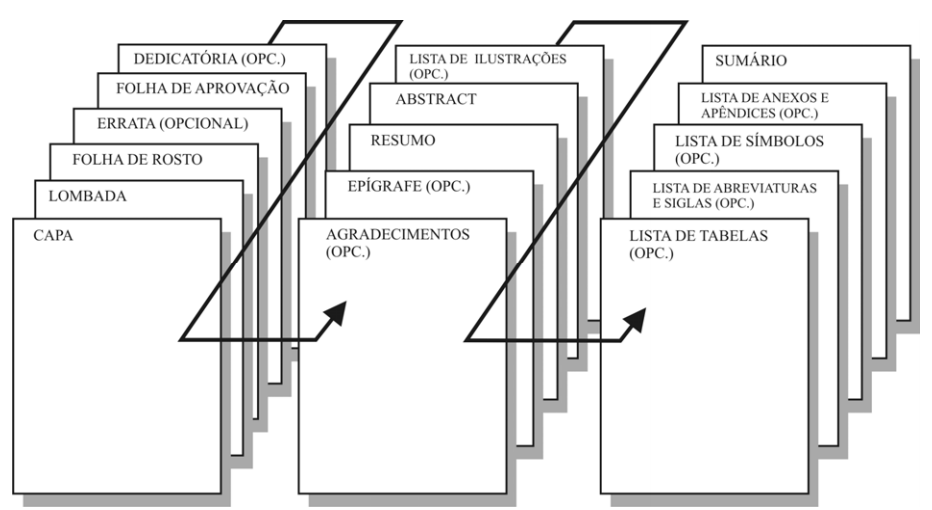
\includegraphics[width=0.6\textwidth]{figuras/pretextuais.png}
	    \vspace{\baselineskip} %%% linha em branco para atendender a norma
            \fonte{Adaptado de \citeonline{man:MDTUFSM2012}.}
         \end{grafico}
         
         
         \section*{Teste de seção dentro do anexo}
